% \vspace{-0.6\baselineskip}
\section{Introduction}
% \vspace{-0.4\baselineskip}
\label{sec:intro}

With the advances of deep learning techniques and increase in dataset scales, there have been successes in scaling up object classification systems. However, unlike object classification, diverse object classes and tedious bounding boxes annotation are hardly scalable. Recently, there have been impressive progresses in unsupervised and weakly supervised object detection, getting rid of the tediou bounding box annotation process. However, existing unsupervised methods show much inferior performance compared to supervised methods. And the weakly supervised ones, which are based on trained on static images, often fail to generalize to videos due to domain shift. In light of this, we investigate the problem of ``weakly supervised object detection by learning from videos''. Instead of using boudning box annotations in fully-supervised pipeline or video-level object class in previous weakly supervised method, we use video-level action class annotation as supervision, as it is easy to obtain and commonly appears in existing video datasets. During training, only videos with action labels are used. As shown in Fig. \ref{fig:train_samples}, the input during evaluation includes static images and both spatial bounding boxes and corresponding object classes are estimated.

\begin{figure}
% \vspace{-0.5\baselineskip}
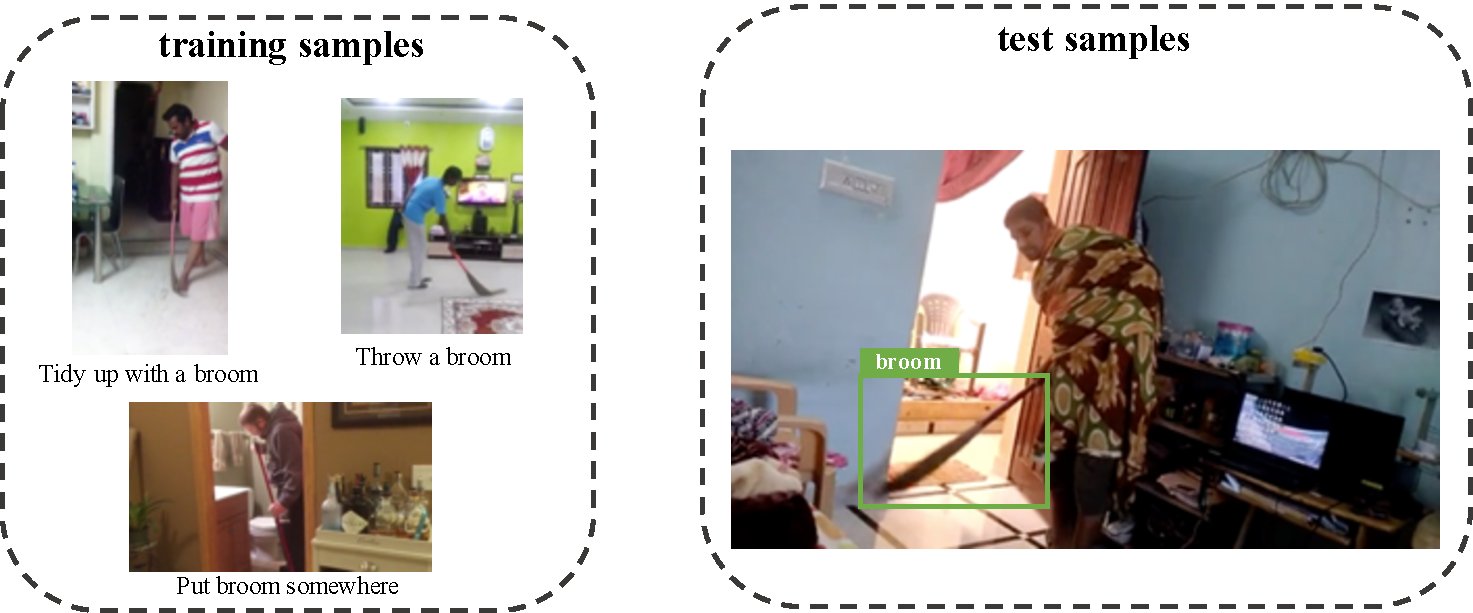
\includegraphics[width=0.5\textwidth]{figures/training_test_samples.pdf}
% \caption{Visual comparison of depth and normal results between \protect\cite{zhou2017unsupervised} and ours. As the original depth ground truth map comes from sparse laser measurement, the interpolated depth map is shown for better visualization. As can be seen from the depth estimation, our results preserve the small/thin structures which have similar color to other foregrounds (green circles). From the normal comparison, our results predict the road normal direction better and have no artifact. The edges in normal map are also preserved better in our results (yello circles).}
\caption{Train samples include videos with action labels. Bounding boxes and object class are estimated during evaluation.}
% \vspace{-0.8\baselineskip}
\label{fig:train_samples}
\end{figure}

Previous work \cite{yuan2017temporal} proposed to cope with problem by leveraging temporal consistency of object proposals and use the object class that appears in the action name (\eg ``cup'' in the action ``drink from cup'') as video-level labels for supervising the learning of object appearance. Specifically, the class-agnostic object proposals are generated using EdgeBoxes \cite{zitnick2014edge}. The proposals are linked in temporal space by measuring the appearance feature similarity. The appearance feature is updated recurrently by incorporating the information from neighboring frames using LSTM. The updated features are further fed into a two-stream classification module as in \cite{bilen2016weakly} and the related object class in action label is used for supervision. Such method failes to model the action motion cues and ignores action class labels, showing 1.98\% mAP on detection task.  

We are motivated by serveral observations: (1) The object appearance is consistent across videos of same action class and also across action classes which involve the same object class; (2) There is spatial correlation between the motions of objects and human key points, \eg in action ``hold cup'', the location of cup is tightly correlated with location of human hand/s. And such correlation is dependent on action class; (3) Action appearance and motion include strong indication for finding the object. Based on these observations, we propose to (1) use human keypoint to help learn the correlation between object motion and actions, (2) apply multiple time-step attention maps to model temporal consistency, (3) jointly learn object classification module and action classification module to leverage the correlation between object appearance and action appearance/motion.


